\section{Continuity} \label{S:1.3.Continuity}

\begin{goals}
\item What does it mean to say that a function $f$ is continuous at $x = a$?  What role do limits play in determining whether or not a function is continuous at a point?
\item What properties do continuous functions have? 
\item How can we use continuous functions?
\end{goals}

%--------------------------------------
% SUBSECTION INTRODUCTION
%--------------------------------------
\subsection*{Introduction}

In Section~\ref{S:1.1.Limits}, we learned about how the concept of limits can be used to study the trend of a function near a fixed input value.  As we study such trends, we are fundamentally interested in knowing how well-behaved the function is at the given point, say $x = a$.  In this present section, we aim to expand our perspective and develop language and understanding to quantify how the function acts and how its value changes near a particular point.  Beyond thinking about whether or not the function has a limit $L$ at $x = a$, we will also consider the value of the function $f(a)$ and how this value is related to $\ds \lim_{x \to a} f(x)$.  Throughout,  we will build on and formalize ideas that we have encountered in several settings.

We begin to consider these issues through the following preview activity that asks you to consider the graph of a function with a variety of interesting behaviors.

\begin{marginfigure}[8cm]
\margingraphics{figures/1_7_PA1.eps}
\caption{The graph of $y = f(x)$.} \label{fig:1.3.PA1}
\end{marginfigure}

\begin{pa} \label{PA:1.3}
A function $f$ defined on $-4 < x < 4$ is given by the graph in Figure~\ref{fig:1.3.PA1}.  Use the graph to answer each of the following questions.  Note: to the right of $x = 2$, the graph of $f$ is exhibiting infinite oscillatory behavior similar to the function $\sin(\frac{\pi}{x})$ that we encountered in the key example early in Section~\ref{S:1.1.Limits}.

\ba
\item For each of the values $a = -3, -2, -1, 0, 1, 2, 3$, determine whether or not $\ds \lim_{x \to a} f(x)$ exists.  If the function has a limit $L$ at a given point, state the value of the limit using the notation $\ds \lim_{x \to a} f(x) = L$.  If the function does not have a limit at a given point, write a sentence to explain why.

\item For each of the values of $a$ from part (a) where $f$ has a limit, determine the value of $f(a)$ at each such point.  

\item For each of the values $a = -3, -2, -1, 0, 1, 2, 3$,  does $f(a)$ have the same value as $\ds \lim_{x \to a} f(x)$?
\ea
\end{pa} 

\afterpa

 % ACTIVITY 

%---------------------------------------
% SUBSECTION CONTINUITY
%---------------------------------------
\subsection*{Being continuous at a point} \index{continuous}

Intuitively, a function is continuous if we can draw it without ever lifting our pencil from the page.  Alternatively, we might say that the graph of a continuous function has no jumps or holes in it.  We first consider three specific situations in Figure~\ref{fig:1-3_Con} where all three functions have a limit at $a = 1$, and then work to make the idea of continuity more precise.

\begin{marginfigure} % MARGIN FIGURE
\captionsetup[subfigure]{labelformat=empty}
\subfloat{\margingraphics{figs/1/1-3_Cona.pdf}}

\subfloat{\margingraphics{figs/1/1-3_Conb.pdf}}

\subfloat{\margingraphics{figs/1/1-3_Conc.pdf}}
\caption{Functions $f$, $g$, and $h$ that demonstrate subtly different behaviors at $a = 1$.}
\label{fig:1-3_Con}
\end{marginfigure}

Note that  $f(1)$ is not defined, which leads to the resulting hole in the graph of $f$ at $a = 1$.  We will naturally say that $f$ is \emph{not continuous at $a = 1$}.  For the next function $g$ in in Figure~\ref{fig:1-3_Con}, we observe that while $\ds \lim_{x \to 1} g(x) = 3$, the value of $g(1) = 2$, and thus the limit does not equal the function value.  Here, too, we will say that $g$ is \emph{not continuous}, even though the function is defined at $a = 1$.  Finally, the function $h$ appears to be the most well-behaved of all three, since at $a = 1$ its limit and its function value agree.  That is,
\[ \lim_{x \to 1} h(x) = 3 = h(1). \]
With no hole or jump in the graph of $h$ at $a = 1$, we desire to say that $h$ is \emph{continuous} there.

More formally, we make the following definition.

\definition{Continuity}{ % DEFINITION
A function $f$ is \emph{continuous} \index{continuous at $x = a$} provided that
\begin{itemize}
\item $f$ has a limit as $x \to a$,
\item $f$ is defined at $x = a$, and
\item $\ds \lim_{x \to a} f(x) = f(a).$
\end{itemize}
A function $f$ is \emph{continuous} on an open interval I if $f$ is continuous at $c$ for all c in I. 

\begin{center}{\large {\bf Continuity at Endpoints}}\end{center}

A function $f$ is continuous at a left-endpoint, $a$, of a closed interval $[a,b]$, or {\em continuous from the right}, if
\[ \lim_{x \to a^+} f(x) = f(a), \]
and $f$ is continuous at a right-endpoint, $b$, of a closed interval $[a,b]$, or {\em continuous from the left}, if
\[ \lim_{x \to b^-} f(x) = f(b), \]
}% end definition

Conditions (a) and (b) are technically contained implicitly in (c), but we state them explicitly to emphasize their individual importance.  In words, (c) essentially says that a function is continuous at $x = a$ provided that its limit as $x \to a$ exists and equals its function value at $x = a$.  Thus, continuous functions are particularly nice:  to evaluate the limit of a continuous function at a point, all we need to do is evaluate the function.

\begin{example}\label{Ex:1.3.Eg1} %%Finding intervals of continuity 
Let $f$ be defined as shown in Figure~\ref{fig:1-3_Eg1}. Give the interval(s) on which $f$ is continuous.

\solution We proceed by examining the three criteria for continuity.
\begin{enumerate}[1)]
\item The limits $\ds \lim_{x \to a} f(x)$ exists for all $a$ between $0$ and $3$.
\item $f(a)$ is defined for all $a$ between $0$ and $3$, \textit{except for} $a=1$. We know immediately that $f$ cannot be continuous at $x=1$.
\item The limit $\ds \lim_{x \to a} f(x) = f(a)$ for all $a$ between $0$ and $3$, except, of course, for $a=1$. 
\item The function is defined at both $x = 0$ and $x = 3$, and both $\ds\lim_{x \to 0^+} f(x) = f(0)$ and $\ds\lim_{x \to 3^-} f(x) = f(3)$.
\end{enumerate}

Therefore, we conclude that $f$ is continuous at every point of $[0,3]$ except at $x=1$. Therefore $f$ is continuous on $[0,1)$ and $(1,3]$.
\end{example}

\begin{marginfigure}[-8cm]
\margingraphics{figs/1/figContinuous1.pdf}
\caption{A graph of $f$ in Example~\ref{Ex:1.3.Eg1}.}\label{fig:1-3_Eg1}
\end{marginfigure} % EXAMPLE 20 1.5 APEX

Let's now consider $p(x) = x^2 - 2x + 3$.  It can be proved that every polynomial is a continuous function at every real number, and thus if we would like to know                                                                                 $\lim_{x \to 2} p(x)$, we simply compute
$$\lim_{x \to 2} (x^2 - 2x + 3) = 2^2 - 2 \cdot 2 + 3 = 3.$$
This route of substituting an input value to evaluate a limit works anytime we know the function being considered is continuous.  Besides polynomial functions, all exponential functions and the sine and cosine functions are continuous at every point, as are many other familiar functions and combinations thereof.  

\begin{example}  % Determining intervals on which a function is continuous.
For each of the following functions, give the domain of the function and the interval(s) on which it is continuous.

\begin{enumerate}[1)]
\item $f(x) = 1/x$			
\item $f(x) = \sin(x)$
\item $f(x) = \sqrt{x}$
\item $f(x) = \sqrt{1-x^2}$
\item $f(x) = |x|$		
\end{enumerate}

\solution We examine each in turn.	
\begin{enumerate}[1)]
\item The domain of $f(x) = 1/x$ is $(-\infty,0) \cup (0,\infty)$. As it is a rational function, we apply the limit laws to recognize that $f$ is continuous on all of its domain.

\item The domain of $f(x) = \sin(x)$ is all real numbers, or $(-\infty,\infty)$. Applying the limit laws shows that $\sin x$ is continuous everywhere.

\item The domain of $f(x) = \sqrt{x}$ is $[0,\infty)$. Applying the limit laws shows that $f(x) = \sqrt{x}$ is continuous on its domain of $[0,\infty)$.

\item The domain of $f(x) = \sqrt{1-x^2}$ is $[-1,1]$. Applying the limit laws shows that $f$ is continuous on all of its domain, $[-1,1]$.

\item The domain of $f(x) = |x|$ is $(-\infty,\infty)$. We can define the absolute value function as $\ds f(x) = \left\{\begin{array}{cc} -x & x<0 \\ x & x\geq 0\end{array}\right.$. Each ``piece'' of this piece-wise defined function is continuous on all of its domain, giving that $f$ is continuous on $(-\infty,0)$ and $[0,\infty)$. As we saw before, we cannot assume this implies that $f$ is continuous on $(-\infty,\infty)$; we need to check that $\ds \lim_{x \to 0}f(x) = f(0)$, as $x=0$ is the point where $f$ transitions from one ``piece'' of its definition to the other. It is easy to verify that this is indeed true, hence we conclude that $f(x) = |x|$ is continuous everywhere.
\end{enumerate}
\end{example} % EXAMPLE 23 1.5 APEX

\begin{marginfigure}[6cm]
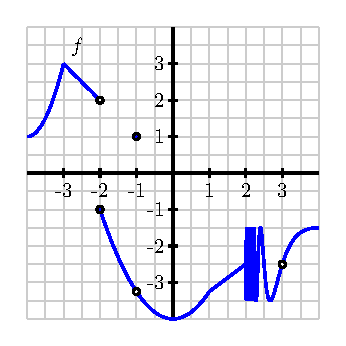
\includegraphics{figures/1_7_PA1.eps}
\caption{The graph of $y = f(x)$ for Activity~\ref{A:1.3.1}.} \label{fig:1-3_A1}
\end{marginfigure}

\begin{activity} \label{A:1.3.1}
This activity builds on your work in Preview Activity~\ref{PA:1.3}, using the same function $f$ as given by the graph that is repeated in Figure~\ref{fig:1-3_A1}.

\ba
	\item At which values of $a$ does $\ds \lim_{x \to a} f(x)$ not exist?
	\item At which values of $a$ is $f(a)$ not defined?
	\item At which values of $a$ does $f$ have a limit, but $\ds \lim_{x \to a} f(x) \ne f(a)$?
	\item State all values of $a$ for which $f$ is not continuous at $x = a$.
	\item Which condition is stronger, and hence implies the other:   $f$  has a limit at $x = a$ or  $f$ is continuous at $x = a$?  Explain, and hence complete the following sentence:  ``If $f$ \underline{\hspace{1.5in}} at $x = a$, then $f$ \underline{\hspace{1.5in}} at $x = a$,'' where you complete the blanks with \emph{has a limit} and \emph{is continuous}, using each phrase once.
\ea
\end{activity}
\begin{smallhint}
\ba
	\item Consider the left- and right-hand limits at each value.
	\item Carefully examine places on the graph where there's an open circle.
	\item Are there locations on the graph where the function has a limit but there's a hole in the graph?
	\item Remember that at least one of three conditions must fail: if the function lacks a limit, if the function is undefined, or if the limit exists but does not equal the function value, then $f$ is not continuous at the point.
	\item Note that the definition of being continuous requires the limit to exist.
\ea
\end{smallhint}
\begin{bighint}
\ba
	\item Consider the left- and right-hand limits at each value, and recall that they must both exist and be equal in order for the overall limit to exist.
	\item Carefully examine places on the graph where there's an open circle; at such locations, look vertically to see if the function has an assigned value at that point.
	\item Are there locations on the graph where the function has a limit but there's a hole in the graph?
	\item Remember that at least one of three conditions must fail: if the function lacks a limit, if the function is undefined, or if the limit exists but does not equal the function value, then $f$ is not continuous at the point.
	\item Note that the definition of being continuous requires the limit to exist.
\ea
\end{bighint}
\begin{activitySolution}
\ba
	\item $\lim_{x \to a} f(x)$ does not exist at $a = -2$ since $\lim_{x \to -2^-} f(x) = 2 \ne -1 = \lim_{x \to -2^+}$ and $\lim_{x \to a} f(x)$ does not exist at $a = +2$ since $\lim_{x \to 2^+} f(x)$ does not exist due to the infinitely oscillatory behavior of $f$.
	\item The only point at which $f$ is not defined is at $a = 3$.
	\item At $x = -1$, note that $\lim_{x \to -1} f(x)$ exists (and appears to have value approximately $-3.25$), but $f(-1) = 1$, and thus $\lim_{x \to -1} f(x) \ne f(-1)$.  At $x = 3$, $\lim_{x \to 3} f(x) = -2.5$, but $f(3)$ is not defined, so the limit exists but does not equal the function value.
	\item Based on our work in (a), (b), and (c), $f$ is not continuous at $a=-2$ and $a = 2$ because $f$ does not have a limit at those points; $f$ is not continuous at $a = 3$ since $f$ is not defined there; and $f$ is not continuous at $a = -1$ because at that point its limit does not equal its function value.
	\item ``If $f$ \underline{is continuous} at $x = a$, then $f$ \underline{has a limit} at $x = a$,'' since one of the defining properties of ``being continuous'' at $x = a$ is that the function has a limit at that input value.  This shows that being continuous is a stronger condition than having a limit.
\ea
\end{activitySolution}
\aftera % ACTIVITY 1.20 in AC 1.7

\begin{activity} \label{A:1.3.2}
State the interval(s) on which each of the following functions is continuous.
\bmtwo
\ba
\item $\ds f(x) = \sqrt{x-1} + \sqrt{5-x}$
\item $\ds f(x) = x\sin(x)$
\item $\ds f(x) = \tan(x)$
\item $\ds f(x) = \sqrt{\ln(x)}$
\ea
\emtwo
\end{activity}
\begin{smallhint}
\ba
	\item Consider the left- and right-hand limits at each value.
	\item Carefully examine places on the graph where there's an open circle.
	\item Are there locations on the graph where the function has a limit but there's a hole in the graph?
	\item Remember that at least one of three conditions must fail: if the function lacks a limit, if the function is undefined, or if the limit exists but does not equal the function value, then $f$ is not continuous at the point.
	\item Note that the definition of being continuous requires the limit to exist.
\ea
\end{smallhint}
\begin{bighint}
\ba
	\item Consider the left- and right-hand limits at each value, and recall that they must both exist and be equal in order for the overall limit to exist.
	\item Carefully examine places on the graph where there's an open circle; at such locations, look vertically to see if the function has an assigned value at that point.
	\item Are there locations on the graph where the function has a limit but there's a hole in the graph?
	\item Remember that at least one of three conditions must fail: if the function lacks a limit, if the function is undefined, or if the limit exists but does not equal the function value, then $f$ is not continuous at the point.
	\item Note that the definition of being continuous requires the limit to exist.
\ea
\end{bighint}
\begin{activitySolution}
\ba
	\item $\lim_{x \to a} f(x)$ does not exist at $a = -2$ since $\lim_{x \to -2^-} f(x) = 2 \ne -1 = \lim_{x \to -2^+}$ and $\lim_{x \to a} f(x)$ does not exist at $a = +2$ since $\lim_{x \to 2^+} f(x)$ does not exist due to the infinitely oscillatory behavior of $f$.
	\item The only point at which $f$ is not defined is at $a = 3$.
	\item At $x = -1$, note that $\lim_{x \to -1} f(x)$ exists (and appears to have value approximately $-3.25$), but $f(-1) = 1$, and thus $\lim_{x \to -1} f(x) \ne f(-1)$.  At $x = 3$, $\lim_{x \to 3} f(x) = -2.5$, but $f(3)$ is not defined, so the limit exists but does not equal the function value.
	\item Based on our work in (a), (b), and (c), $f$ is not continuous at $a=-2$ and $a = 2$ because $f$ does not have a limit at those points; $f$ is not continuous at $a = 3$ since $f$ is not defined there; and $f$ is not continuous at $a = -1$ because at that point its limit does not equal its function value.
	\item ``If $f$ \underline{is continuous} at $x = a$, then $f$ \underline{has a limit} at $x = a$,'' since one of the defining properties of ``being continuous'' at $x = a$ is that the function has a limit at that input value.  This shows that being continuous is a stronger condition than having a limit.
\ea
\end{activitySolution}
\aftera % ACTIVITY 

%----------------------------------------------------------
% SUBSECTION INTERMEDIATE VALUE THEOREM
%----------------------------------------------------------
\subsection*{Intermediate Value Theorem}

This intuitive notion of continuity does help us understand another important concept as follows. Suppose $f$ is defined on $[1,2]$ and $f(1) = -10$ and $f(2) = 5$. If $f$ is continuous on $[1,2]$ (i.e., its graph can be sketched as a continuous line from $(1,-10)$ to $(2,5)$) then we know intuitively that somewhere on $[1,2]$ $f$ must be equal to $-9$, and $-8$, and $-7,\ -6,\ \ldots,\ 0,\ 1/2,$ etc. In short, $f$ takes on all \textit{intermediate} values between $-10$ and $5$. It may take on more values; $f$ may actually equal 6 at some time, for instance, but we are guaranteed all values between $-10$ and $5$. 

While this notion seems intuitive, it is not trivial to prove and its importance is profound. Therefore the concept is stated in the form of a theorem.

\concept{Intermediate Value Theorem}{% CONCEPT
Let $f$ be a continuous function on $[a,b]$ and, without loss of generality, let $f(a) < f(b)$. Then for every value $y$, where $f(a) < y < f(b)$, there is a value $c$ in $[a,b]$ such that $f(c) = y$. 
}% end concept

One important application of the Intermediate Value Theorem is root finding. Given a function $f$, we are often interested in finding values of $x$ where $f(x) = 0$. These roots may be very difficult to find exactly. Good approximations can be found through successive applications of this theorem. Suppose through direct computation we find that $f(a) <0 $ and $f(b)>0$, where $a<b$. The Intermediate Value Theorem states that there is a $c$ in $[a,b]$ such that $f(c) = 0$. The theorem does not give us any clue as to where that value is in the interval $[a,b]$, just that it exists. 

There is a technique that produces a good approximation of $c$. Let $d$ be the midpoint of the interval $[a,b]$ and consider $f(d)$. There are three possibilities:
\begin{enumerate}[1)]
\item $f(d) = 0$ -- we got lucky and stumbled on the actual value. We stop as we found a root.
\item $f(d) <0$ Then we know there is a root of $f$ on the interval $[d,b]$ -- we have halved the size of our interval, hence are closer to a good approximation of the root.
\item $f(d) >0$ Then we know there is a root of $f$ on the interval $[a,d]$ -- again,we have halved the size of our interval, hence are closer to a good approximation of the root.
\end{enumerate}
	
Successively applying this technique is called the \emph{Bisection Method} \index{Bisection Method} of root finding. We continue until the interval is sufficiently small. We demonstrate this in the following example.

\begin{marginfigure}[6cm]
\margingraphics{figs/1/figXMinusCosX.pdf} 
\caption{Graphing a root of $f(x) = x-\cos(x)$.}\label{fig:1-3_Eg3}
\end{marginfigure}

\begin{margintable}
\scalebox{1.1}{
\begin{tabular}{ccc}
Iteration \# & Interval & Midpoint Sign \\ \hline
			1 & $[0.7,0.9]$ & $f(0.8) >0$ \\
			2 & $[0.7,0.8] $ & $f(0.75) >0$ \\
			3 & $[0.7,0.75]$ & $f(0.725)<0$\\
			4 & $[0.725,0.75]$ & $f(0.7375)<0$\\
			5 & $[0.7375,0.75]$ & $f(0.7438)>0$\\
			6 & $[0.7375,0.7438]$ & $f(0.7407)>0$\\
			7 & $[0.7375,0.7407]$ & $f(0.7391)>0$\\
			8 & $[0.7375,0.7391]$ & $f(0.7383)<0$\\
			9 & $[0.7383,0.7391]$ & $f(0.7387)<0$\\
			10 & $[0.7387,0.7391]$ & $f(0.7389)<0$\\
			11 & $[0.7389,0.7391]$ & $f(0.7390)<0$\\
			12 & $[0.7390,0.7391]$ &   \\
\end{tabular}
} % end scalebox 
\caption{Iterations of the Bisection Method of Root Finding}\label{T:1-3_Eg3}
\end{margintable}

\begin{example}   %Using the Bisection Method 
Approximate the root of $f(x) = x-\cos x$, accurate to three places after the decimal.

\solution Consider the graph of $f(x) = x-\cos x$, shown in Figure~\ref{fig:1-3_Eg3}. It is clear that the graph crosses the $x$-axis somewhere near $x=0.8$. To start the Bisection Method, pick an interval that contains $0.8$. We choose $[0.7,0.9]$. Note that all we care about are signs of $f(x)$, not their actual value, so this is all we display.

\begin{description}
\item[Iteration 1:] $f(0.7) < 0$, $f(0.9) > 0$, and $f(0.8) >0$. So replace $0.9$ with $0.8$ and repeat.
\item[Iteration 2:] $f(0.7)<0$, $f(0.8) > 0$, and at the midpoint, $0.75$, we have $f(0.75) >0 $. So replace $0.8$ with $0.75$ and repeat. Note that we don't need to continue to check the endpoints, just the midpoint. Thus we put the rest of the iterations in Table~\ref{T:1-3_Eg3}.
\end{description}

Notice that in the $12^{\text{th}}$ iteration we have the endpoints of the interval each starting with $0.739$. Thus we have narrowed the zero down to an accuracy of the first three places after the decimal. Using a computer, we have 
\[ f(0.7390) = -0.00014, \quad f(0.7391) = 0.000024. \] 
Either endpoint of the interval gives a good approximation of where $f$ is $0$. The Intermediate Value Theorem states that the actual zero is still within this interval. While we do not know its exact value, we know it starts with $0.739$. 

This type of exercise is rarely done by hand. Rather, it is simple to program a computer to run such an algorithm and stop when the endpoints differ by a preset small amount. One of the authors did write such a program and found the zero of $f$, accurate to $10$ places after the decimal, to be $0.7390851332$. While it took a few minutes to write the program, it took less than a thousandth of a second for the program to run the necessary $35$ iterations. In less than $8$ hundredths of a second, the zero was calculated to $100$ decimal places (with less than $200$ iterations).
\end{example}
 % EXAMPLE

It is a simple matter to extend the Bisection Method to solve similar problems to $f(x) = 0$. For instance, we can solve $f(x) = 1$. This may seem obvious, but to many it is not. It actually works very well to define a new function $g$ where $g(x) = f(x) - 1$. Then use the Bisection Method to solve $g(x)=0$.  

Similarly, given two functions $f$ and $g$, we can use the Bisection Method to solve $f(x) = g(x)$. Once again, create a new function $h$ where $h(x) = f(x)-g(x)$ and solve $h(x) = 0$. 

\begin{activity} \label{A:1.3.3}
Use the Bisection Method to approximate, accurate to two decimal places, the value of the root of the given functions and intervals.

\ba
\item $\ds f(x) = x^2 + 2x - 4; \quad [1,1.5]$
\item $\ds f(x) = e^x - 2; \quad [0.65, 0.7]$
\ea
\end{activity}

\aftera % ACTIVITY 

%--------------
% SUMMARY
%--------------
\begin{summary}
%\item A function $f$ has limit $L$ as $x \to a$ if and only if $f$ has a left-hand limit at $x = a$, has a right-hand limit at $x = a$, and the left- and right-hand limits are equal.  Visually, this means that there can be a hole in the graph at $x = a$, but the function must approach the same single value from either side of $x = a$.
\item A function $f$ is continuous at $x = a$ whenever $f(a)$ is defined, $f$ has a limit as $x \to a$, and the value of the limit and the value of the function agree.  This guarantees that there is not a hole or jump in the graph of $f$ at $x = a$.

\item We can use the Intermediate Value Theorem to determine if there may be a root of a continuous function on a closed interval.
%\item A function $f$ is differentiable at $x = a$ whenever $f'(a)$ exists, which means that $f$ has a tangent line at $(a,f(a))$ and thus $f$ is locally linear at the value $x = a$.  Informally, this means that the function looks like a line when viewed up close at $(a,f(a))$ and that there is not a corner point or cusp at $(a,f(a))$. 
%\item Of the three conditions discussed in this section (having a limit at $x = a$, being continuous at $x = a$, and being differentiable at $x = a$), the strongest condition is being differentiable, and the next strongest is being continuous.  In particular, if $f$ is differentiable at $x = a$, then $f$ is also continuous at $x = a$, and if $f$ is continuous at $x = a$, then $f$ has a limit at $x = a$.
\end{summary}

\clearpage

%--------------
% EXERCISES
%--------------
\begin{adjustwidth*}{}{-2.25in}
\textbf{{\large Exercises}}
\setlength{\columnsep}{25pt}
\begin{multicols*}{2}
\noindent Terms and Concepts \small

\begin{enumerate}[1)]
\item {In your own words, describe what it means for a function to be continuous.}
\item {In your own words, describe what the Intermediate Value Theorem states.}
\item {What is a ``root'' of a function?}
\item {Given functions $f$ and $g$ on an interval $I$, how can the Bisection Method be used to find a value $c$ where $f(c) = g(c)$?}
\item {T/F:	If $f$ is defined on an open interval containing $c$, and $\ds \lim_{x\to c}f(x)$ exists, then $f$ is continuous at $c$.}
\item {T/F: If $f$ is continuous at $c$, then $\ds \lim_{x\to c}f(x)$ exists.}
\item {T/F: If $f$ is continuous at $c$, then $\ds \lim_{x\to c^+}f(x) = f(c)$.}
\item {T/F: If $f$ is continuous on $[a,b]$, then $\ds\lim_{x\to a^-}f(x) = f(a)$.}
\item {T/F: If $f$ is continuous on $[0,1)$ and $[1,2)$, then $f$ is continuous on $[0,2)$.}
\item {T/F: The sum of continuous functions is also continuous.}
\end{enumerate} 

\noindent {\normalsize Problems\\} \small

\noindent In exercises 11--17, a graph of $f$ is given along with a value $a$.  Determine if $f$ is continuous at $a$; if it is not, state why it is not.

\begin{enumerate}[1),resume]
\item
{\noindent $a = 1$

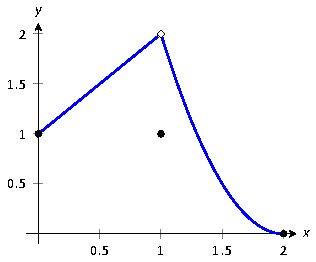
\includegraphics[scale=.8]{figures/fig01_04_ex_05}
}

\item
{\noindent $a = 1$

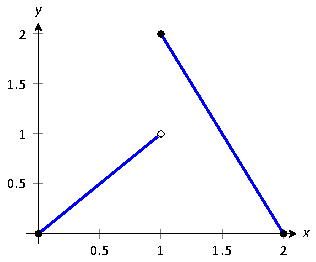
\includegraphics[scale=.8]{figures/fig01_04_ex_06}
}

\vspace{.5cm}

\item
{\noindent $a = 1$

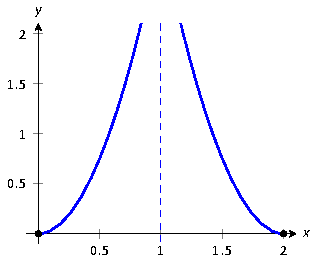
\includegraphics[scale=.8]{figures/fig01_04_ex_07}
}

\item
{\noindent $a = 0$

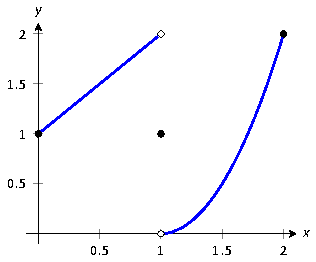
\includegraphics[scale=.8]{figures/fig01_04_ex_08}
}

\item
{\noindent $a = 1$

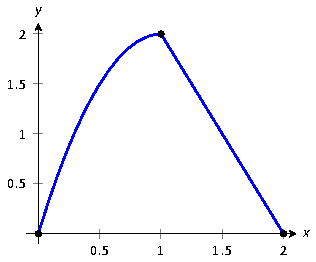
\includegraphics[scale=.8]{figures/fig01_04_ex_09}
}

\item
{\noindent $a = 4$

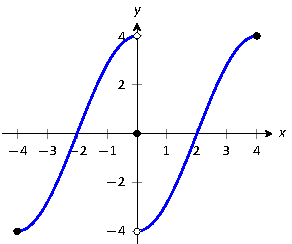
\includegraphics[scale=.8]{figures/fig01_04_ex_10}
}

\item
{\begin{enumerate}
\item		$a = -2$
\item		$a=0$
\item		$a=2$
\end{enumerate}

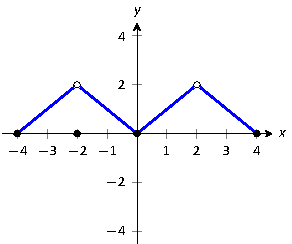
\includegraphics[scale=.8]{figures/fig01_04_ex_11}
}

\end{enumerate}

\vspace{.5cm}

%------------------------------------------
% END OF EXERCISES ON FIRST PAGE
%------------------------------------------
\end{multicols*}
\end{adjustwidth*}

\clearpage

\begin{adjustwidth*}{}{-2.25in}
\setlength{\columnsep}{25pt}
\begin{multicols*}{2}\small

In exercises 18--21, determine if $f$ is continuous at the indicated values.  If not, explain why.

\begin{enumerate}[1),start=18]
\item 
{$\ds f(x) = \left\{\begin{array}{ccc} 
1		& & x=0\\
\ds\frac{\sin(x)}{x} & & x>0
\end{array}\right.
$
\begin{enumerate}
\item		$x=0$
\item		$x=\pi$
\end{enumerate}
}

\item 
{$\ds f(x) = \left\{\begin{array}{ccc} 
x^3-x		& & x<1\\
x-2 & & x\geq 1
\end{array}\right.
$
\begin{enumerate}
\item		$x=0$
\item		$x=1$
\end{enumerate}
}

\item 
{$\ds f(x) = \left\{\begin{array}{ccc} 
\ds\frac{x^2+5x+4}{x^2+3x+2}		& &  x\neq -1\\
3 & & x=-1
\end{array}\right.
$
\begin{enumerate}
\item		$x=-1$
\item		$x=10$
\end{enumerate}
}

\item
{$\ds f(x) = \left\{\begin{array}{ccc}
\ds\frac{x^2-64}{x^2-11 x+24}		& &  x\neq 8\\
5 & & x=8
\end{array}\right.
$
\begin{enumerate}
\item		$x=0$
\item		$x=8$
\end{enumerate}
}
\end{enumerate}

\vspace{.5cm}

\noindent In exercises 22--32, give the intervals on which the given function is continuous.

\begin{enumerate}[1),start=22]
\item $\ds f(x) = x^2-3x+9$
\item $\ds g(x) = \sqrt{x^2-4}$
\item $\ds h(k) = \sqrt{1-k}+\sqrt{k+1}$
\item $\ds f(t) = \sqrt{5t^2-30}$
\item $\ds g(t) = \frac{1}{\sqrt{1-t^2}}$
\item $\ds g(x) = \frac{1}{1+x^2}$
\item $\ds f(x) = e^x$
\item $\ds g(s) = \ln s$
\item $\ds h(t) = \cos(t)$
\item $\ds f(k) = \sqrt{1-e^k}$
\item $\ds f(x) = \sin(e^x+x^2)$
\end{enumerate}

\vspace{.5cm}

\noindent In exercises 33--34, use the Bisection Method to approximate, accurate to two decimal places, the value of the root of the given function in the given interval.

\begin{enumerate}[1),start=33]
\item $\ds f(x) = \sin(x) - \frac{1}{2}; \quad [0.5, 0.55]$
\item $\ds f(x) = \cos(x) - \sin(x); \quad [0.7, 0.8]$
\end{enumerate}

%---------------------------------------------
% END OF EXERCISES ON SECOND PAGE
%---------------------------------------------
\end{multicols*}
\end{adjustwidth*}
\afterexercises 

\cleardoublepage